\header{2}
\chapter{Bootonderdelen \& Zeiltermen}
\section{Inleiding}
In dit hoofdstuk komen de verschillende onderdelen van de boot en een aantal zeiltermen aan bod. Deze termen en onderdelen zijn belangrijk om de volgende hoofdstukken goed te begrijpen.

\section{Zeiltermen}
Voor duidelijke communicatie tijdens de les en in de boot is het van belang dat je een aantal zeiltermen kent. De belangrijkste termen worden hieronder besproken.

\subsection{Bakboord, Stuurboord, Loef en Lij}
Bakboord en stuurboord zijn het links en rechts \textbf{van de boot}, gezien vanaf het achterdek. Je moet altijd met de vaarrichting mee kijken. Loef en lij zeggen iets over de wind ten opzichte van je boot. De kant waar de wind de boot in komt, is de loefzijde, ook wel de hoge kant genoemd. De kant waar de wind de boot verlaat heet de lijzijde of lage kant. De hogerwal is de wal waar de wind vandaan komt. De lagerwal is de wal waar de wind naar toe waait. Al deze termen zijn te zien in figuur \ref{pic:hoog_laag}. 
\begin{figure}[ht]
	\centering
	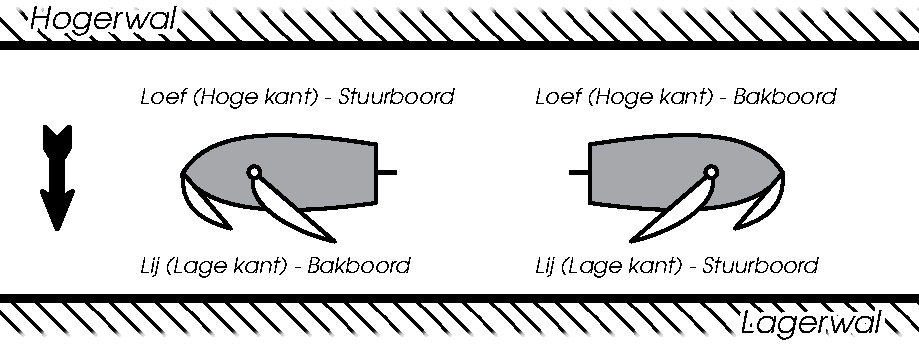
\includegraphics[width=0.8\textwidth]{Hoofdstukken/Onderdelen/pdf/wallen.pdf}
	\caption{Hoger- en Lagerwal}
	\centering
	\label{pic:hoog_laag}
\end{figure}

\subsection{Boven- en benedenwinds}
\begin{figure}[H]
	\centering
	\begin{minipage}[t]{0.55\textwidth}
		\vspace{-4cm}
		Op het water kan je vaak op twee manieren ergens langs varen: bovenwinds en benedenwinds. Bovenwinds houdt in dat je ergens langs vaart aan de kant waar de wind ernaartoe blaast, de hoge kant van het object. Benedenwinds is het tegenovergestelde: dit is de kant waar de wind van het object weg blaast en dus de lage kant van het object. Deze termen zijn te zien in figuur \ref{pic:boven_benedenwinds}.
	\end{minipage}
	\hfill
	\begin{minipage}[b]{0.40\textwidth}
		\centering
		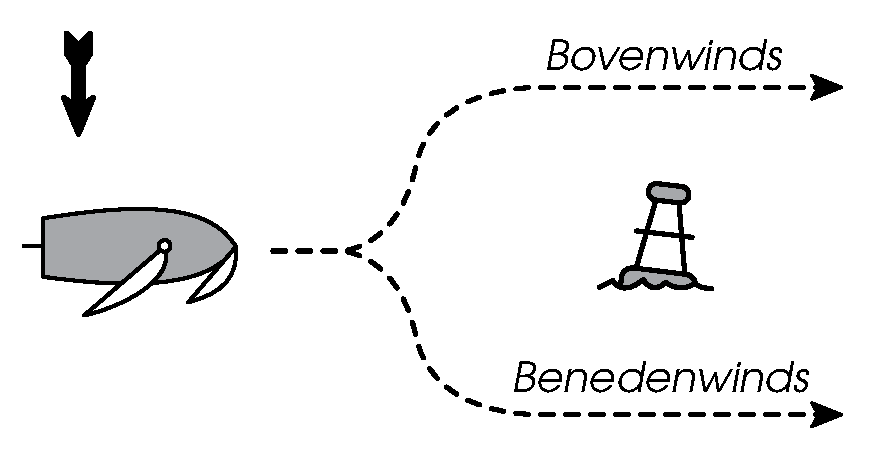
\includegraphics[width=\textwidth]{Hoofdstukken/Onderdelen/pdf/boven_en_benedenwinds.pdf}
		\caption{}
		\centering
		\label{pic:boven_benedenwinds}
	\end{minipage}
\end{figure}

\vfil\newpage

\subsection{Koersen}
Een koers vertelt iets over hoe je boot ligt ten opzichte van de wind. Alle koersen kun je zowel over bakboord, als stuurboord varen, behalve in de wind. Een overzicht van de koersen is te zien in figuur \ref{pic:koersen}. Wanneer je van koers verandert en naar de wind toe draait, loef je op. Wanneer je van de wind wegdraait heet dit afvallen. 

\begin{figure}[h]
	\centering
	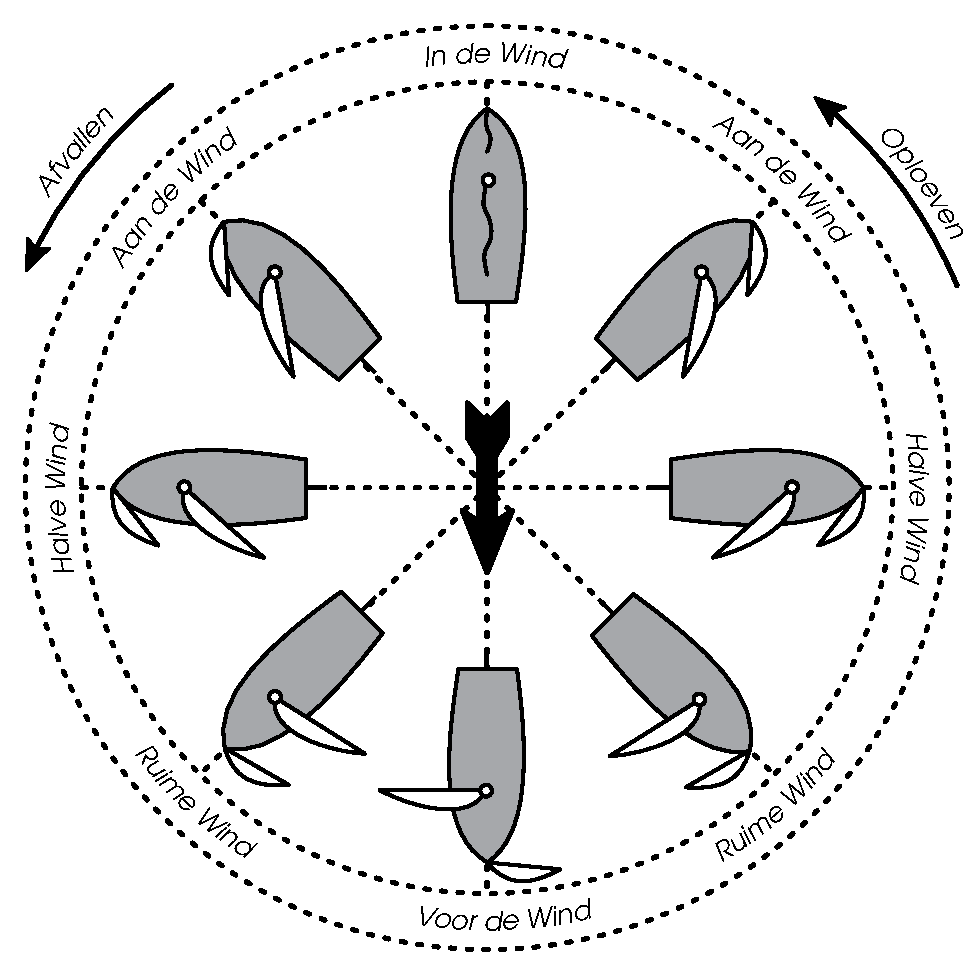
\includegraphics[width=0.9\textwidth]{Hoofdstukken/Onderdelen/pdf/koersen.pdf}
	\caption{Windkoersen}
	\label{pic:koersen}
\end{figure}


\subsection{Overstag en opkruisen}
Wanneer je overstag gaat, ga je van aan de wind over de ene boeg naar aan de wind over de andere boeg. Bijvoorbeeld van aan de wind over bakboord naar aan de wind over stuurboord. Door meerdere malen achter elkaar overstag te gaan kun je naar een punt zeilen dat tegen de wind in ligt. Dit heet opkruisen of laveren en is te zien in figuur \ref{pic:opkruisen}. Het stuk wat je aan de wind vaart de tussen twee overstagen noem je een slag.  

In figuur \ref{pic:kort_lang} ligt het vaarwater niet exact in de wind, maar komt de wind met een kleine hoek naar binnen. Hierdoor zijn de slagen niet meer van gelijke lengte. Er is dan spraken van een korte slag en een lange slag.

\begin{figure}[h]
	\centering
	\begin{minipage}{0.40\textwidth}
		\centering
		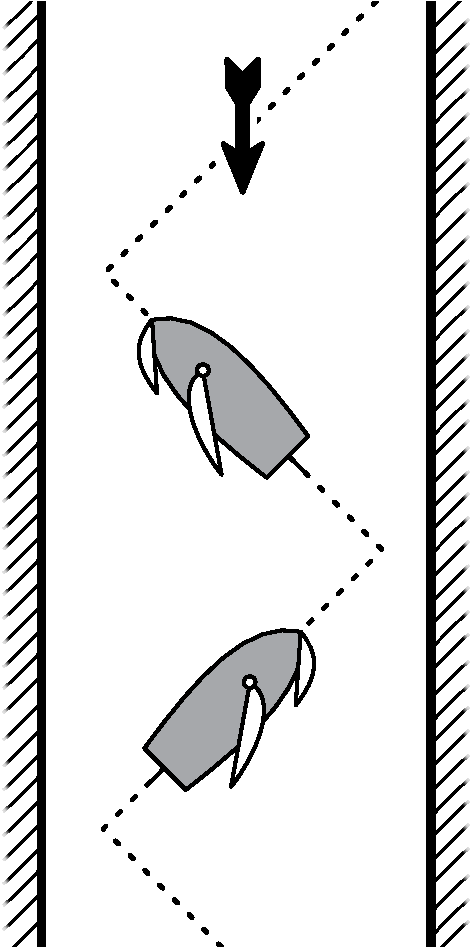
\includegraphics[width=0.6\textwidth]{Hoofdstukken/Onderdelen/pdf/opkruisen.pdf}
		\caption{Opkruisen}
		\centering
		\label{pic:opkruisen}
	\end{minipage}
	\begin{minipage}{0.40\textwidth}
		\centering
		\includegraphics[width=0.6\textwidth]{Hoofdstukken/Onderdelen/pdf/korte_lange_Slag.pdf}
		\caption{Korte en Lange Slag}
		\label{pic:kort_lang}
	\end{minipage}
\end{figure}

\newpage

Door gebruik te maken van deze verschillende slaglengtes kun je zo effectief mogelijk opkruisen. In de korte slag probeer je zo veel mogelijk snelheid te maken. Vaar hier desnoods wat lager aan de wind om extra snelheid te maken. Deze snelheid gebruik je vervolgens in je lange slag. In deze slag probeer je zo veel mogelijk hoogte te winnen. Door scherp aan de wind te varen en de gewonnen snelheid uit de korte slag te gebruiken, leg je de meeste meters af.

\subsection{Gijpen en `binnen de wind varen'}
\begin{figure}[H]
	\centering
	\begin{minipage}[t]{0.78\textwidth}
		\vspace{-5cm}
		Gijpen kun je ook wel beschouwen als het tegenovergestelde van een overstag. Je gaat hier namelijk van voor de wind over de ene boeg naar voor de wind over de andere boeg. Bijvoorbeeld van voor de wind over bakboord naar voor de wind over stuurboord. Als je de gijp en de overstag in de windroos in figuur \ref{pic:koersen} plaatst zie je dat ze precies tegenover elkaar liggen.\\
		
		
		Door vlak voor het gijpen iets extra af te vallen, gijpt je zeil eenvoudiger. Dit extra afvallen is te zien in figuur \ref{pic:binnen_wind}. De onderste boot vaart exact voor de wind. De bovenste boot vaart richting ruime wind over stuurboord, maar met zijn zeil nog aan bakboord. Dit heet `binnen de wind' varen.
	\end{minipage}
	\hfill
	\begin{minipage}[b]{0.18\textwidth}
		\centering
		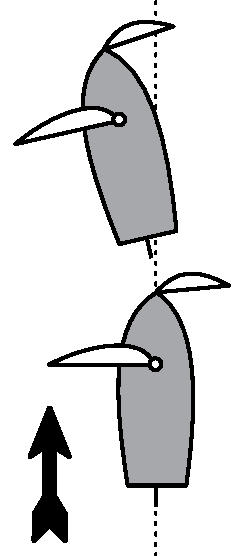
\includegraphics[width=0.7\textwidth]{Hoofdstukken/Onderdelen/pdf/binnen_de_wind.pdf}
		\caption{}
		\label{pic:binnen_wind}
	\end{minipage}
\end{figure}


\subsection{Overig}
Hiernaast dien je ook bekend te zijn met de onderstaande termen:

\begin{itemize}
	
	\item \textit{Bezeild}: Wanneer een punt bezeild kan worden, kan je hier komen zonder op te kruisen. 
	\item \textit{Planeren}: Wanneer een boot planeert vaart deze op zijn eigen boeggolf. De boot gaat niet meer door het water heen, maar glijdt er overheen. 
	\item \textit{Volvallen}: Volvallen definieert de boeg waarover je weg zeilt als je in de wind stil gelegen hebt. Als je volvalt over bakboord is je grootzeil aan bakboord bij het wegvaren.
	\item \textit{Verhalen}: Wanneer een schip verhaalt wordt, wordt deze over een korte afstand verplaatst door bomen, wrikken of door het gebruik van lijnen.
	\item \textit{Verlijeren of Drift}: Verlijeren of drift is de zijwaartse snelheid die een schip krijgt door de wind. 	
	\item \textit{Opschieter}: Bij een hogerwal aanleggen door vlak voor de kant de neus van de boot in de wind te draaien en zo al je snelheid te verliezen.
	\item \textit{Dwarspeiling}: Met een dwarspeiling maak je een inschatting van de koers die je zult varen na een overstag.
	\item \textit{Bijliggen}: Tijdens het bijliggen wordt de fok bak gezet en opgeloeft met het roer. Hierdoor dobbert de boot tussen in de wind en halve wind in. Het roer en fok kunnen eventueel vast worden gezet.
	\item \textit{Killen van het zeil}: Je laat dan expres een deel van je zeil minder wind vangen. Dit doe je door je zeil te vieren totdat alleen het achterlijk nog wind vangt.
	\item \textit{Bak}: Wanneer je je fok bak doet, zet je deze aan de hoge kant in plaats van de lage kant.
	\item \textit{Deinzen}: Dit is wanneer je achteruit dobbert met de neus van je boot in de wind.
\end{itemize}


\section{Bootonderdelen}
In figuur \ref{pic:vlet_nummers} is een tekening van een lelievlet te zien met maar liefst 88 gelabelde onderdelen. De namen van de onderdelen staan in tabel \ref{table:vletwel}. Alle onderdelen, behalve die met grijze nummers, moet je kennen.

\begin{table}[h!]
\centering
\caption{Vletonderdelen}

\setlength\extrarowheight{5pt} %Add height to center text vertically
\renewcommand{\arraystretch}{0.75} %Shrink total heigt to keep row same heigt
\newcommand{\tabhead}[1]{\cellcolor{ocre}{\color[HTML]{FFFFFF}\sffamily \textbf{#1}}}
\newcommand{\NIL}[1]{\cellcolor{not}{#1}}
\label{table:vletwel}

\begin{tabular}{|ll|ll|ll|ll|}
	\multicolumn{2}{|l|}{\tabhead{Fok}}       & \multicolumn{2}{l|}{\tabhead{Grootzeil}}   & \multicolumn{2}{l|}{\tabhead{Lopend want}} & \multicolumn{2}{l|}{\tabhead{Casco}}  \\
	\textbf{1}           & Fok               & \textbf{24}      & Zeilteken              & \textbf{45}        & Fokkeschoot          & \textbf{68}     & Doft               \\
	\textbf{2}           & Tophoek           & \textbf{25}      & Zeilnummer             & \textbf{46}        & Grootschoot          & \textbf{\NIL69} & Dofthouder         \\
	\textbf{3}           & Halshoek          & \textbf{26}      & Zeillat                & \multicolumn{2}{l|}{\tabhead{Casco}}      & \textbf{70}     & Vlonder/Denning    \\
	\textbf{4}           & Schoothoek        & \textbf{\NIL27}  & Baan                   & \textbf{47}        & Dolboord             & \textbf{71}     & Spant              \\
	\textbf{5}           & Voorlijk          & \multicolumn{2}{l|}{\tabhead{Gaffel}}     & \textbf{48}        & Boeisel              & \multicolumn{2}{l|}{\tabhead{Zwaard}} \\
	\textbf{\NIL6}       & Achterlijk        & \textbf{28}      & Gaffel                 & \textbf{49}        & Berghout             & \textbf{72}     & Zwaard             \\
	\textbf{\NIL7}       & Onderlijk         & \textbf{29}      & Spruit/gaffeldraad     & \textbf{50}        & Boeg                 & \textbf{73}     & Zwaardbout         \\
	\textbf{\NIL8}       & Leuver            & \textbf{\NIL 30} & Strop                  & \textbf{52}        & Vlak                 & \textbf{74}     & Zwaardloper        \\
	\multicolumn{2}{|l|}{\tabhead{Mast}}     & \textbf{31}      & Klauw                  & \textbf{53}        & Scheg                & \textbf{75}     & Zwaardgreep        \\
	\textbf{9}           & Mast              & \textbf{32}      & Marllijn               & \textbf{54}        & Spiegel              & \textbf{76}     & Zwaardpen          \\
	\textbf{10}          & Windvaantje       & \multicolumn{2}{l|}{\tabhead{Giek}}       & \textbf{55}        & Voordek              & \textbf{77}     & Zwaardkast         \\
	\textbf{\NIL11}      & Mastring          & \textbf{33}      & Giek                   & \textbf{56}        & Achterdek            & \textbf{78}     & Zwaardplaatje      \\
	\textbf{12}          & Rijglijn          & \textbf{34}      & Lummelbeslag           & \textbf{57}        & Kim                  & \textbf{79}     & Mastkoker          \\
	\textbf{13}          & Mastbout          & \textbf{35}      & Grootschootring        & \textbf{58}        & Luchtkast            & \textbf{80}     & Kikker             \\
	\textbf{14}          & Grendelbout       & \textbf{36}      & Wervel                 & \textbf{59}        & Hanenkam             & \multicolumn{2}{l|}{\tabhead{Roer}}   \\
	\multicolumn{2}{|l|}{\tabhead{Grootzeil}}& \textbf{37}      & Pettenlijntje          & \textbf{60}        & Sleepoog             & \textbf{81}     & Helmstok           \\
	\textbf{15}          & Grootzeil         & \multicolumn{2}{l|}{\tabhead{Staand want}}& \textbf{\NIL61}        & Hijsoog              & \textbf{82}     & Roerkoning         \\
	\textbf{16}          & Tophoek           & \textbf{38}      & Voorstag               & \textbf{\NIL62}    & Leioog               & \textbf{83}     & Roerhaak           \\
	\textbf{17}          & Klauwhoek         & \textbf{39}      & Zijstag                & \textbf{\NIL63}    & Grootschootoog       & \textbf{84}     & Roerblad           \\
	\textbf{18}          & Halshoek          & \textbf{\NIL 40} & Voorstagspanner        & \textbf{\NIL 64}   & Landvastoog          & \textbf{85}     & Vingerling         \\
	\textbf{19}          & Schoothoek        & \multicolumn{2}{l|}{\tabhead{Lopend want}}& \textbf{\NIL65}    & Wrikgat              & \multicolumn{2}{l|}{\tabhead{Vlag}}   \\
	\textbf{\NIL20}      & Bovenlijk         & \textbf{41}      & Fokkeval               & \textbf{66}        & Dol                  & \textbf{\NIL86}  & Vlag               \\
	\textbf{21}          & Voorlijk          & \textbf{42}      & Klauwval               & \textbf{67}        & Dolpot               & \textbf{\NIL87}  & Vlaggenstok        \\
	\textbf{22}          & Achterlijk        & \textbf{43}      & Piekeval               & \textbf{}          &                      & \textbf{\NIL88}  & Knop               \\
	\textbf{\NIL23}      & Onderlijk         & \textbf{44}      & Kraanlijn / dirk       & \textbf{}          &                      & \textbf{}       &                    \\ \hline
\end{tabular}

\setlength\extrarowheight{0pt} %Reset
\renewcommand{\arraystretch}{1} %Reset

\end{table}
\newpage
\begin{figure}[h!]
    \centering
    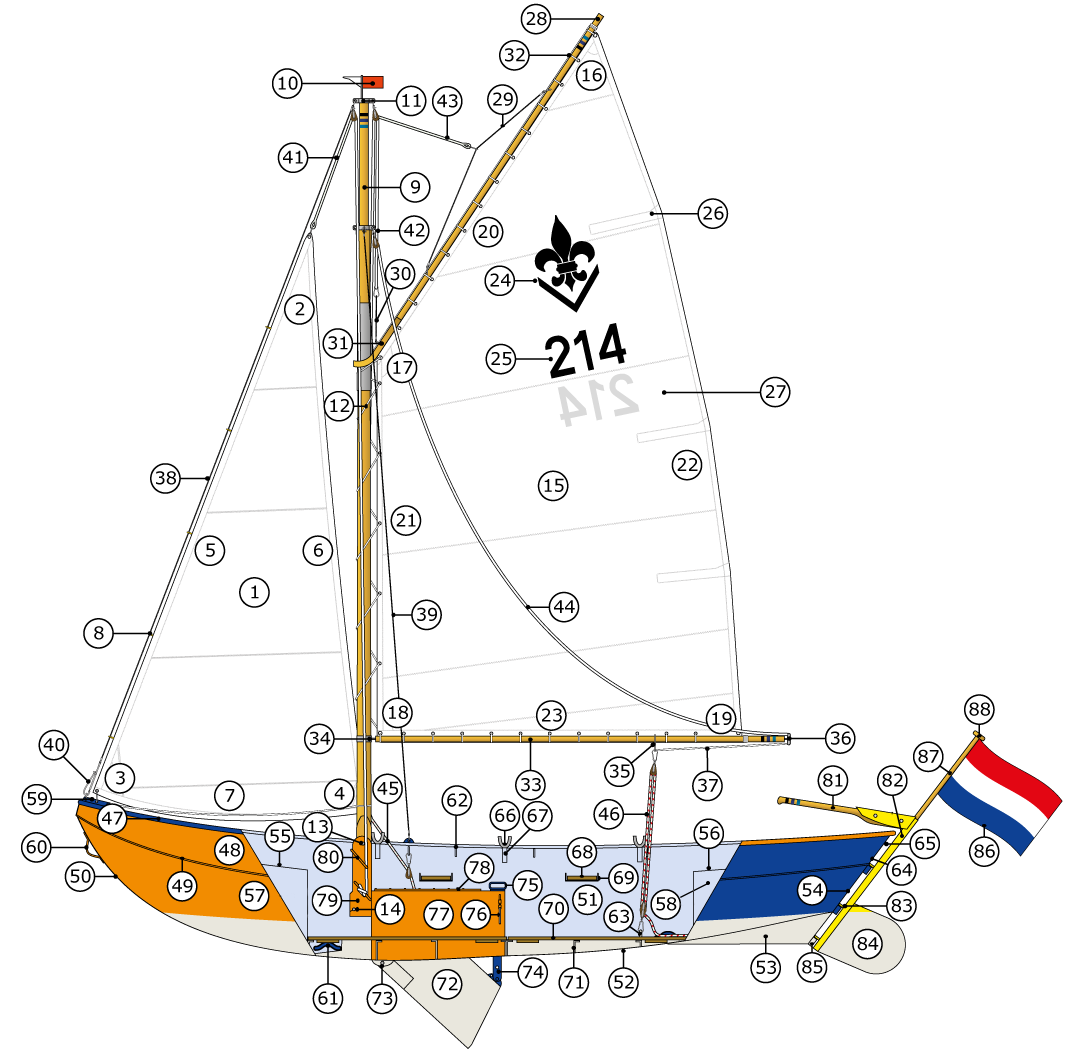
\includegraphics[width=1.15\textwidth]{Hoofdstukken/Onderdelen/png/lelievlet_onderdelen.png}
    \caption{Tekening lelievlet met nummers \protect\footnotemark}
    \centering
    \label{pic:vlet_nummers}
\end{figure}
\footnotetext{\textit{Lelievlet\_onderdelen.png}, https://www.willibrordusgroep.nl/Images/upload/cwo/lelievlet\_onderdelen.png, Feb 2021.
}

\subsection{Extra onderdelen}
\label{ss:extra}
Niet alle onderdelen zijn uit te beelden in figuur \ref{pic:vlet_nummers}. Deze extra onderdelen zijn daarom hieronder toegelicht.
\vspace*{-0.2cm}
\begin{itemize}
	\item \textit{Voorsteven}: Voorkant van een boot of boeg.
	\item \textit{Sluiting}: Middel om lijnen mee te bevestigen. Voorbeeld: harpje of musketon haak.
	\item \textit{Kous}: Verstevigd metalen oog in het zeil.
	\item \textit{Kiel}: Steekt onder de bodem van het schip uit en voorkomt verlijeren en geeft stabiliteit.
	\item \textit{Halstalie}: Blok en lijn waarmee de halshoek naar beneden gespannen kan worden.
\end{itemize}

\newpage

\section{Conclusie}
Naast dat je nu bekend bent met de bootonderdelen uit tabel \ref{table:vletwel} en de extra onderdelen uit paragraaf \ref{ss:extra},  zijn dit al de zeiltermen uit de vorige paragrafen die je kent en begrijpt.
\begin{itemize}[label=]
\begin{multicols}{4}
	\item Bakboord
	\item Stuurboord
	\item Loefzijde
	\item Lijzijde
	\item Hoge kant
	\item Lage kant
	\item Hogerwal
	\item Lagerwal
	\item In de wind
	\item Aan de wind
	\item Halve wind
    \item Ruime wind
    \item Voor de wind
    \item Oploeven
    \item Afvallen
    \item Bovenwinds
    \item Benedenwinds
    \item Overstag gaan
    \item Opkruisen
    \item Korte slag
    \item Lange slag
    \item Gijpen
    \item Binnen de wind
    \item Bezeild
    \item Planeren
    \item Volvallen
    \item Verhalen
    \item Verlijeren
    \item Drift
    \item Opschieter
    \item Dwarspeiling
    \item Bijliggen
    \item Killen van het zeil 
    \item Bak
    \item Deinzen
\end{multicols}
\end{itemize}